%!TEX root = ../dokumentation.tex

\subsection{Publisher und Subscriber}
\label{subsec:pubsub}

Das \ac{Pub/Sub} Paradigma wird in der Literatur als asynchroner, nachrichtenorientierter Service bezeichnet (vgl. \cite{XinZhang}, S.1). Der Service ermöglicht, es zwei Komponenten miteinander kommunizieren zu lasssen. Die Komponenten sind auf der einen Seite ein Data Producer, auch Publisher genannt und auf der Gegenseite der Data Consumer, Subscriber.
\\Beim \acs{Pub/Sub} verhält sich die Kommunikation datenzentriert, das bedeutet, dass die Verwaltung und die Verteilung der geschickten Daten im Vordergrund steht (vgl. \cite{Salehi2018}).
\\Der grundsätzliche Ablauf der Kommunikation besteht aus dem Veröffentlichen einer Nachricht vom Publisher, ohne zu wissen, wer diese Nachricht lesen wird. Der Gegenspieler zum Publisher ist der Subscriber, welcher Nachrichten über einen Kanal entgegennimmt ohne direktes Wissen über den Publisher dieser Nachricht (vgl. \cite{Salehi2018}).
Duch die Trennung der sendenden Komponente und der empfangenden Komponente wird dem System eine lose Kopplung und Skalierbarkeit zugesprochen (vgl. \cite{Salehi2018}).

Auch \acs{Redis} bietet den Service \acs{Pub/Sub} an. Im Kontext von \acs{Redis} ist \acs{Pub/Sub} ein stabiles Messaging Model, welches eine schnelle Kommunikation zwischen ein oder mehreren Nutzern erlaubt (vgl. \cite{Nelson2016}, S.56).
Hierbei können Publisher Nachrichten in spezifischen Kanälen veröffentlichen, welche von Subscribern des Kanals empfangen werden (vgl. \cite{Redis-PubSub}). Die Interaktion läuft hierbei immer mit einem einzigen Publisher ab, jedoch können auf der Subscriber Seite eine Vielzahl an Usern die Nachricht empfangen.
In \acs{Redis} stehen die Teilnehemer einer Kommunikation nicht im direkten Kontakt. Die Kommunikation wird über einen Broker, also über einen Vermittler abgehandelt, bei \acs{Redis} ist dies ein Knoten in einem verteilten System (vgl. \cite{Redis-PubSub}).

\acs{Pub/Sub} in \acs{Redis} ist nicht mit dem \textit{key-space}, also dem Namenraums, in dem alle Schlüssel abgelegt werden, verbunden. Die von einem Publisher veröffentlichten Nachrichten werden nicht persistiert und können daher auch nur von Subscribern wahrgenommen werden, wenn sie zum Zeitpunkt der Veröffentlichung mit dem System verbunden sind. 
Daher wird \acs{Pub/Sub} in dieser From auch als \textit{at most once message delivery} Service bezeichnet (vgl. \cite{Redis-PubSub}). Nachrichten werden nur einmal vom \acs{Redis}-Server an alle Subscriber in Form eines Broadcast gesendet, wenn ein Subscriber aufgrund von einem Fehler die Nachricht nicht verarbeiten kann, ist diese für immer verloren und kann nicht wiederhergestellt werden. 

Das Format der Übertragung an die einzelnen Clients, die zu einem Kanal subscribed sind ist im allgemeinen ein \textit{wire protocol}. Mit dieser Art der Übertragung können Daten von einem \textit{Redis-Server} an einen \textit{Redis-Client} übertragen werden.
In \acs{Redis} wird diese Übertragung spezielle \textit{Redis-Protocol} genannt (vgl. \cite{Redis-PubSub}).
Das \textit{Redis-Protocol} kann in \acs{Pub/Sub} als ein Array wahrgenommen werden mit drei Elementen. Das erste Element bezeichnet die Art der Nachricht, das zweite den Kanal in dem die Nachricht veröffentlicht wurde und das dritte Element ist der Inhalt der Nachricht. 

Das Beispiel in \autoref{fig:wire} beschreibt, wie ein Array mit 3 Elementen an den Client geschickt wird. Das erste Element ist sieben Zeichen lang und es handelt sich um den Inhalt \glqq message\grqq, um zu Signalisieren, dass eine Nachricht empfangen wird. Gefolgt wird die Nachricht mit einem Element der Zeichenlänge sechs und dem Inhalt \glqq second\grqq, was der Kanalname ist, in dem die Nachricht veröffentlicht wird. Zuletzt wird ein fünf Zeichen langes Element gesendet, welches den tatsächlichen Inhalt der Nachricht darstellt: \glqq Hello\grqq.
Die Nachricht aus dem Beispiel wird nur von den Clients verarbeitet, die den Kanal \textit{second} subscribed haben.
\begin{figure}[h]
	\centering
	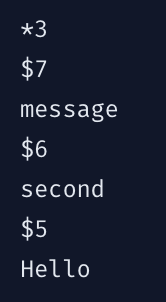
\includegraphics[width=0.15\textwidth]{images/wire_protocol.png}
	\caption{Wire-Protocol Beispiel (vgl. \cite{Redis-PubSub})}
	\label{fig:wire} 
\end{figure}

Subscriber sind in ihrer Anzahl an Kanälen nicht limitiert. In \acs{Redis} besteht sogar die Möglichkeit eine sogenannte \textit{pattern matching subscribtion} abzuschließen. Diese Art der Subscribtion erlaubt des einem \textit{Redis-Client} alle Kanäle zu empfangen, die ein bestimmtes Namensmuster haben. Besipielsweise können mit \textit{PSUBSCRIBE news.*} alle Nachrichten empfangen werden, die in den Kanälen mit dem Präfix \textit{news} veröffentlicht werden.


\subsection{Security}
\label{subsection:security}
\acs{Redis} wurde mit dem Gedanken konzipiert, dass nur zugelassenen Clients in einer vertrauten Umgebung  Zugriff auf \acs{Redis}-Instanzen gewährt wird. 
Im Allgemeinen ist es nicht ratsam, \acs{Redis} in einer Umgebung einzusetzen, in der direkte Zugriffe über das Internet erfolgen und unvertrauenswürdige Clients Zugriff auf den \acs{Redis} \ac{TCP}-Port haben könnten (vgl. \cite{Redis-Security}).

In Situationen, in denen \textit{Caching} für Webseiten erforderlich ist und potenziell unvertrauenswürdige Clients die Anwendung nutzen, sollte der Zugriff auf Redis nicht direkt vom Client erfolgen. Stattdessen wird dies über die Anwendung selbst ausgeführt, die als Vermittler dient.
Hierbei können \acp{ACL} eingesetzt werden, um Benutzereingaben zu validieren und zu entscheiden, welche Aktionen erlaubt sind. Die Authentifizierung der Clients erfolgt hierbei auch über die \acp{ACL}.
Diese können mit Passwörtern als zusätzliche Schutzmaßnahme verwendet werden, falls Firewalls oder andere Sicherheitsmaßnahmen nicht ausreichen. Der Client muss das Passwort kennen, um Zugriff zu erhalten (vgl. \cite{Redis-Security}).

Obwohl \ac{TLS} von \ac{Redis} unterstützt wird, ist es optional. Es kann auf den Kommunikationskanälen zwischen Nodes, Clients, Replikas und auch auf dem \acs{Redis} Cluster Bus Protokoll implementiert werden (vgl. \cite{Redis-Security}).

Eine zusätzliche Sicherheitsmaßnahme besteht darin, Befehle unbrauchbar zu machen, indem man sie umbenennt. Zum Beispiel könnte der Konfigurationsbefehl (\textit{CONFIG}) in einen Hex-Code umbenannt werden. Dies trägt dazu bei, potenzielle Sicherheitslücken zu minimieren und eine sicherere \acs{Redis}-Umgebung zu schaffen (vgl. \cite{Redis-Security}).
